\section{Beispielseite: Kontakt}

\textsc{Matthias Vongerichten}

\begin{figure}[h]
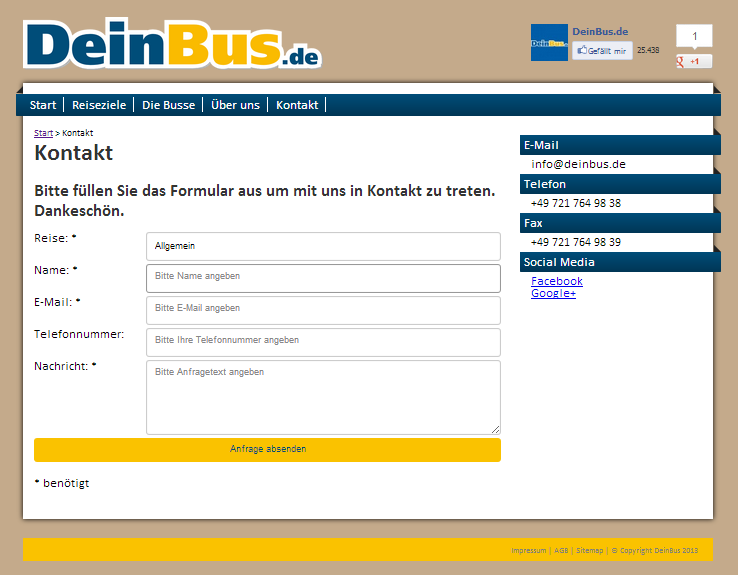
\includegraphics[width=\hsize]{scr_kontakt}
\caption{Screenshot: Kontaktformular}
\label{scr:kontakt}
\end{figure}

Die Seite "`Kontakt"' besteht zum gr��ten Teil aus einem Kontaktformular und den alternativen Kontaktm�glichkeiten in der Sidebar. 

Das Kontaktformular verwendet das �bliche HTML-Tag "`Form"' sowie einige HTML5-Funktionen. Erkennbar ist dies z.B. an dem Attribut "`required"', welches dem Browser signalisiert, dass dieses Formularelement ausgef�llt werden muss. Versucht der Benutzer das Formular abzuschicken erh�lt er einen Hinweis �ber das leere Element und wird aufgefordert es auszuf�llen - vorausgesetzt der Browser ist HTML5-kompatibel. Das Formular wird wie in Abbildung ~\ref{abb:formular} gezeigt durch eine �bliche Tabelle strukturiert (HTML-Table Tag).

\begin{figure}[h]
\begin{minted}[bgcolor=bg]{html}
<tr>
   <td>Name: *</td>
   <td>
      <input id          ="name"  
             placeholder ="Bitte Name angeben" 
             type        ="text" 
             tabindex    ="1" 
             required 
             autofocus
      >
   </td>
</tr>
\end{minted}
\caption{Quellcode: Formular (HTML)}
\label{abb:formular}
\end{figure}

F�r den Fall einer fehlenden HTML5-Unterst�tzung wurde eine Fallback-L�sung mittels JavaScript implementiert. Die Pr�fung auf eine HTML5-Unterst�tzung wurde wie wie in Abbildung ~\ref{abb:required} gezeigt umgesetzt und wird bei jedem Abschicken des Formulars durchgef�hrt.

\begin{figure}[h]
\begin{minted}[bgcolor=bg]{javascript}
var inputs = document.createElement('input');
var supports = {};
supports.required  = 'required' in inputs;

if(!supports.required) {
   /*...siehe unten...*/
}
\end{minted}
\caption{Quellcode: HTML5 oder JavaScript--Fallback (JavaScript)}
\label{abb:required}
\end{figure}

Trifft die Pr�fung zu und HTML5 wird nicht unterst�tzt wird jedes auszuf�llende Formularelement auf dessen Inhalt gepr�ft. Bei einem Fehler wird die Formular�bermittlung abgebrochen und der Fokus auf das betroffene Element gesetzt (Siehe Abbildung ~\ref{abb:fokus}).

\begin{figure}[h]
\begin{minted}[bgcolor=bg]{javascript}
name = document.getElementById("name").value;
/*...*/
if (name == "")
{
   document.getElementById("name").select();
   document.getElementById("name").focus();
   return false;
}
\end{minted}
\caption{Quellcode: Fokussteuerung bei fehlerhaften Eingaben (JavaScript)}
\label{abb:fokus}
\end{figure}

Da HTML5 auch die Plausibilit�t von E-Mail-Adressen pr�ft wurde auch dies im Fallback mit einer entsprechenden Abfrage ber�cksichtigt (Siehe Abbildung ~\ref{abb:test}). 

\begin{figure}[h]
\begin{minted}[bgcolor=bg]{javascript}
if (!checkEmail(email))
{
   alert('E-Mail ist ung�ltig.');
   return false;
}
\end{minted}
\caption{Quellcode: Abfrage: E--Mail Adresse g�ltig? (JavaScript)}
\label{abb:test}
\end{figure}

In der darin aufgerufenen Funktion wurde mithilfe des regul�ren Ausdrucks in Abbildung ~\ref{abb:regex} auf eine g�ltige E--Mail Adresse getestet

\begin{figure}[h]
\begin{minted}[bgcolor=bg]{javascript}
function checkEmail(inputvalue) {
   var pattern = /^([a-zA-Z0-9_\.\-])\
                  +\@(([a-zA-Z0-9\-])+\.)\
                  +([a-zA-Z0-9]{2,4})+$/;
   return pattern.test(inputvalue);
}
\end{minted}
\caption{Quellcode: Regul�rer Ausdruck: E--Mail Adresse (JavaScript)}
\label{abb:regex}
\end{figure}
